\documentclass{article}
\usepackage[utf8]{inputenc}

\title{Compulsory Assignment 1}
\author{isakhammer }
\date{2020}

%
%
%%%% DEPENDENCIES v1.5 %%%%%%

\usepackage{natbib}
\usepackage{graphicx}
\usepackage{amsmath}
\usepackage{amsthm}
\usepackage{amsfonts}
\usepackage{mathtools}
%\usepackage{enumerate}
\usepackage{enumitem}
\usepackage{todonotes}
\usepackage{esint}
\usepackage{float}

\usepackage{mathrsfs}

\usepackage{hyperref}
\hypersetup{
    colorlinks=true, %set true if you want colored links
    linktoc=all,     %set to all if you want both sections and subsections linked
    linkcolor=blue,  %choose some color if you want links to stand out
}
\hypersetup{linktocpage}


% inscape-figures
\usepackage{import}
\usepackage{pdfpages}
\usepackage{transparent}
\usepackage{xcolor}
\newcommand{\incfig}[2][1]{%
\def\svgwidth{#1\columnwidth}
\import{./figures/}{#2.pdf_tex} } \pdfsuppresswarningpagegroup=1

% Box environment
\usepackage{tcolorbox}
\usepackage{mdframed}
\newmdtheoremenv{definition}{Definition}[section]
\newmdtheoremenv{theorem}{Theorem}[section]
\newmdtheoremenv{lemma}{Lemma}[section]

\DeclareMathOperator{\atantwo}{atan2}
\DeclareMathOperator{\arctantwo}{arctan2}

\theoremstyle{remark}
\newtheorem*{remark}{Remark}
%\newtheorem{example}{Example}

\newcommand{\newpara}
    {
    \vskip 0.4cm
    }

%%%%%%%%%%%%%%%%%%%%%%%%%%%%%%%%%%%%%%%%%%%%%%%%%%%%%%%%%%%%

%

%

\begin{document}
\maketitle
\tableofcontents
\newpage

\newpage
\section*{Problem 1}%
\label{sec:problem_1}

Let $\mu = E\left( X \right) = \begin{pmatrix}
0 \\
2
\end{pmatrix}
$
and $\Sigma  = cov \left( X \right) = \begin{pmatrix}
3 & 1 \\
1 & 3
\end{pmatrix}
$
s.t. \[
Y = \begin{pmatrix}
Y_{1} \\
Y_{2}
\end{pmatrix}
= \begin{pmatrix}
\frac{1}{\sqrt{2} } & -  \frac{1}{\sqrt{2} } \\
\frac{1}{\sqrt{2} } &  \frac{1}{\sqrt{2} }
\end{pmatrix}X
\]

\subsection*{ 1a}%
\label{sub:_a}

\begin{enumerate}[label=(\roman*)]
    \item We want to find the mean vector and the covariance vector of $Y$.
        \[
        E\left( Y \right) = E\left( AX \right) = AE\left( X \right) = \begin{pmatrix}
    -\frac{2}{\sqrt{2} } \\
    \frac{2}{\sqrt{2} }
    \end{pmatrix}
        \]

    \[
        \begin{split}
        cov\left( Y \right)  &=  cov \left( AX \right) = A cov\left( X \right) A^{T} \\
        &=  \begin{pmatrix}
        2 & 0 \\
        0 & 4
        \end{pmatrix}
         \\
        \end{split}
    \]
\item The distribution of $Y$ is a bivariate normal distribution, where \[
Y \sim  N\left( E\left( Y \right), cov\left( Y \right) \right)
\]
\item We can observe that $Y_{1}$ and $Y_{2}$  is independent since \[
cov \left( Y_{1}, Y_{2} \right) = 0
\]
\end{enumerate}


\subsection*{ 1b}%
\label{sub:1_b}


Let the pdf be given as the equation of a ellipse s.t. \[
\begin{split}
    f\left( x \right)  = a,& \quad  a>0 \\
    \left( x- \mu  \right)^{T} \Sigma ^{-1} \left( x - \mu  \right) & = b.
\end{split}
\]

The relation of $b$  and $a$ can be derived as follows,\[
    \begin{split}
f\left( x \right) & = k \cdot  \exp \left( - \left( x- \mu  \right)^{T} \Sigma \left( x - \mu  \right) \right) = a \\
\ln k - \ln a &=  \left( x- \mu  \right)^{T} \Sigma  \left( x-\mu  \right) \\
    \end{split}
\]

Thus $b = \ln k - \ln a$, where $\displaystyle k = \frac{1}{2 \pi \left| \Sigma  \right|}$. Clearly, can we observe that
the aligment of the ellipse is oriented along the eigenvectors of $\Sigma $ . Furthermore, the half lengths is described by the
scalar $b$  and eigenvalues \[
    l_{1} = \sqrt{b} \sqrt{\lambda _{1}}  \quad \text{and} \quad  \sqrt{b}  \sqrt{\lambda _{2}} .
\]
Since $\left( x- \mu  \right) \Sigma ^{-1} \left( x - \mu  \right)$ is a sum of normal distributed variables can we
compute the probability a random variable being inside the ellipse $\alpha $ by using the fact that \[
    \left( x - \mu   \right)^{-1} \Sigma  \left( x - \mu  \right) \sim  \chi _{2} ^{2}.
\]

Hence, the probability can be computed using $\chi _{2}^{2}\left( \alpha   \right) \le b \iff \alpha  \approx 0.9$.



\begin{figure}[H]
    \centering
    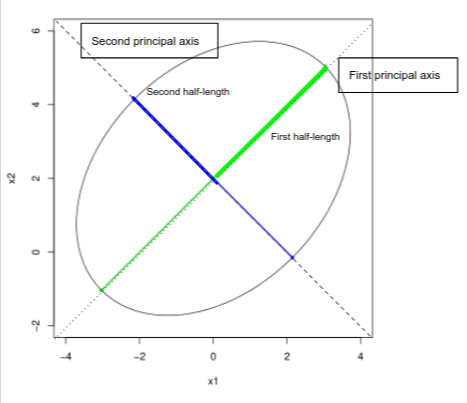
\includegraphics[width=0.7\textwidth]{axis.png}
    \label{oppg3}
\end{figure}


\newpage
\section*{Problem 2}%
\label{sec:problem_2}

\subsection*{2a}%
\label{sub:2a}
Let  $ X= [ X_{1}, X_{2}, X_{3}, \ldots , X_{n} ]^{T}$ be a stochastic vector and a vector of ones $\mathbf{1} = \mathbf{1}_{n \times  1}$ .
\begin{enumerate}[label=(\roman*)]
    \item \[
\overline{X} = \frac{1}{n} \sum_{i=1}^{n}  X_{i} = \frac{1}{n}\mathbf{1}^{T}\left[ X_{1}, \ldots, X_{n}
        \right]^{T}  = \frac{1}{n}\mathbf{1}^{T}  X
    \]
\item  \[
\begin{split}
    S^{2} & = \frac{1}{\left( n-1 \right)} X^{T } CX  = \frac{1}{\left( n-1 \right)} X^{T} C C X \\
    &=  \frac{1}{\left( n-1 \right)} \left( CX \right)^{T} \left( CX \right) \\
    &=  \frac{1}{\left( n-1 \right)} \left( X- \mathbf{1} \overline{X}  \right)^{T} \left( X- \mathbf{1} \overline{X}  \right)\\
    &=  \frac{1}{\left( n-1 \right)} \sum_{i=1}^{n} \left( X_{i} - \overline{X}  \right)\left( X_{i} - \overline{X}  \right) \\
\end{split}
\]
\end{enumerate}



\subsection*{2b}%
\label{sub:2b}

We want to show the independence of $\overline{X} $  and $S^{2}$. Firstly,  we want to emphasis the result that \[
      \displaystyle  \frac{1}{n} \mathbf{1} ^{T} \left( C \right) = \frac{1}{n} \mathbf{1}^{T} \left( I -
        \frac{\mathbf{1}\mathbf{1}^{T}}{n} \right) = \frac{1}{n} \mathbf{1}^{T} - \frac{1}{n} \mathbf{1}^{T} = 0
\]

We will utilize the fact that \[
    cov\left( \overline{X} , S^{2} \right) = cov\left( \frac{1}{n} \mathbf{1^{T}} X, C X \right)  = \frac{1}{n}
    \mathbf{1^{T}} \sigma I C = \sigma \cdot 0.
\]

Hence $\overline{X} $ and $S^{2}$ are independent.






\newpage
\section{References}%
\label{sec:references}

\bibliographystyle{plain}
\bibliography{references}
\end{document}

